\documentclass[journal]{IEEEtran}

\usepackage{graphicx} 
\usepackage{caption} 
\usepackage{siunitx} 
\usepackage{subcaption} 
\captionsetup[table]{skip=10pt}
\usepackage[margin=1in]{geometry} 
\usepackage{amsmath,amsthm,amssymb}
\usepackage[noend]{algpseudocode}
\usepackage{algorithm2e}
\usepackage[section]{placeins}
\usepackage{float}
\makeatletter
\def\BState{\State\hskip-\ALG@thistlm}
\makeatother
\captionsetup{font=footnotesize}
\DeclareMathOperator{\atantwo}{atan2}

\graphicspath{{media/}}

\begin{document}

\title{Team 9 ROB 550 BotLab}

\author{Peter Mitrano, Nathaniel Cox, Sidhartha Dey}

\maketitle

\begin{abstract}
    This report documents the ROB 550 Botlab project. The goal of this project was to create the necessary algorithms for a 3-DOF mobile robot to autonomously map a two-dimensional region while simultaneously localization and planning optimal paths. Students learned about motion and sensor models with probabilistic distributions, Monte Carlo localization, occupancy grid mapping and A* search to enable simultaneous localization and mapping (SLAM) and path planning. 
\end{abstract}
\IEEEpeerreviewmaketitle

\section{Introduction}
\IEEEPARstart{I}{n} this report, we discuss the methods, results and observations implemented and made for the ROB 550  Team 9 Botlab project. Using a 3-DOF mobile robot, we employed several Robotics Engineering topics with the goal of creating a system to autonomously map a region while simultaneously localizing and planning optimal paths. Topics included: motion and sensor models with probabilistic distributions, Monte Carlo localization, occupancy grid mapping, Simultaneous Localization and Mapping (SLAM), and A* search path planning. The mobile robot system consisted of two DC motors equip with encoders to enable differential driving and odometry, lidar to map surroundings, and an inertial measurement unit (IMU) to correct headings. We tested and observed our final system as part of a course competition with three primary events. 

Our report is organized with five primary sections: Methods implemented to complete the project and the results we observed are provided in sections II and III, while observations regarding performance and possible improvements are discussed in section IV.

\section{Methodology}

    In order to perform basic navigation in a static environment, we developed and tested algorithms for SLAM, exploration, path planning, and waypoint following. The role of SLAM is to determine the position of the robot within the world, and to determine which cells are occupied, unoccupied, or unknown. Using this, our exploration algorithm selects cells to navigate to. Next, our path planning algorithm determines a series of waypoints that form the shortest collision free path to that cell. Finally, we control the forward and rotational velocity of the robot to reach these waypoints in succession. In the following sections, we describe how we implemeted each of the components.
    
    \subsection{Simultaneous Localization and Mapping (SLAM)}
    
        SLAM is a well established class of algorithms which generally involve an iterative process of building a map and localizing to that map. Figure \ref{fig:sys} shows a block diagram of how our specific SLAM implementation works. They key functions of our implementation include Bresenham's algorithm to ray trace beams and find occupied and free cells and a particle filter to estimate our pose. Within the particle filter, we used an action model based on odometry to propagate the particles, and a sensor model to weight the particles.
        
        \begin{figure}[b]
            \centering
            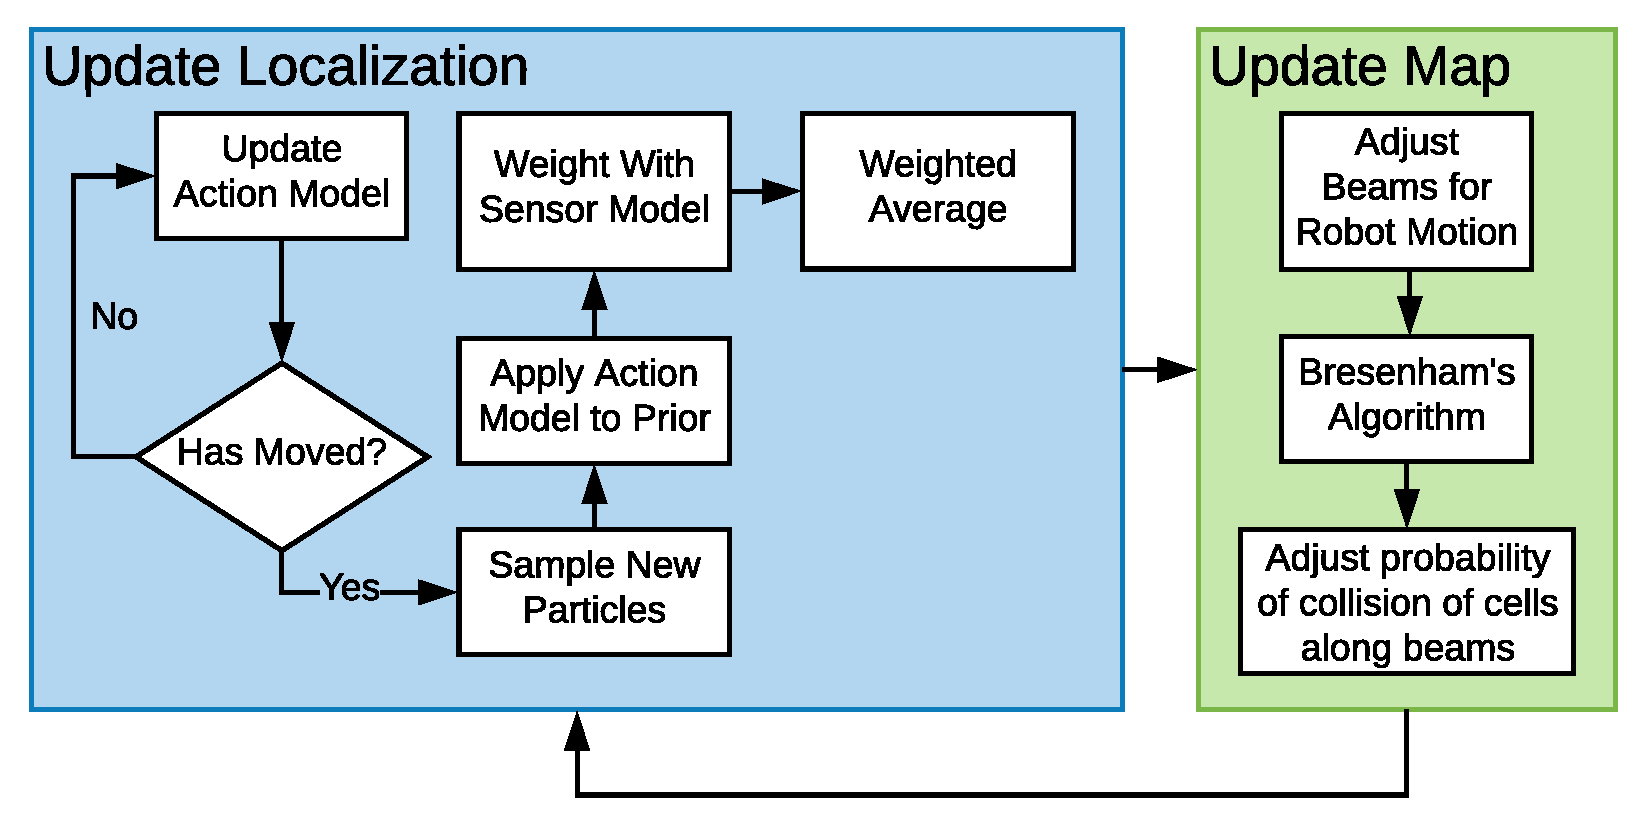
\includegraphics[width=1\linewidth]{slam.pdf}
            \caption{System diagram}
            \label{fig:sys}
        \end{figure}
    
        \subsubsection{Mapping}
        
        We implemented an occupancy grid mapping algorithm to produce a map identifying occupied regions where the robot could not navigate. Our map allowed for a \SI{10}{\meter} x \SI{10}{\meter} region, discretized into \SI{5}{\centi\meter} cells. We represented the occupancy of each cell using the log-odds, with an initially unexplored map holding cells of log-odds zero (equal probability of occupied and vacant).
        Each time our robot performed a lidar scan of the local region, we implemented Bresenham’s line algorithm \cite{lecture12} to determine through which cells the ray traversed. From the unique cells, we created a vector to store the cell indices to determine for which cells the ray terminated (hit) and which the ray passed through (miss). For the last cell of this vector, we applied a hit log-odds constant of 3 and for all other cells we a applied a miss log-odds constant of -1. We then added the new log-odds based on the hit or miss to the previously found log-odds to update the map.

        \subsubsection{Monte Carlo Localization}
            
            % ASSIGNED: Sid
            
            Monte Carlo Localization (MCL) is a well-known localization method used in mobile robots \cite{Fox99Mon}. Unlike state estimation methods like the Kalman filter, the essence of MCL is the particle filter, a non-parametric method to represent the probability distribution of the robot's position and orientation, called the state of the robot. Here, each particle is an estimated pose of the robot and the distribution of particles represents the probability distribution of the estimation. 
            The Monte Carlo Localization algorithm can be broken down into 3 steps: (1) predicting the next pose for each particle by applying a motion based on the action commands sent to the robot and a model of the robots motion, called the action model. (2) computing a weight for each particle which corresponds to the probability of the robot having that predicted pose given a sensor reading and a model of the robot's sensor, aptly called the sensor model. (3) resampling the particles or poses based on their weights, thus phasing out state estimations which were less likely to occur and focusing on the more probable poses without having to add more particles. 
        
        \subsubsection{Action Model}
            \label{ssec:action_model}
            
            % TODO: Revise the action model you described. 
            We implemented the sampling\_motion\_model\_odometry described by Thrun, Burgard and Fox \cite{Prob_Rob}. We chose to use the odometry model over the velocity model as it is, in general, more accurate than the velocity model, even though odometry suffers from error accumulation over time. \cite{Prob_Rob} presents two odometry algorithms - \texttt{motion\_model\_odometry}, which predicts the probability of action $u_{t}$ leading to state $x_{t}$ and is represented as $p(x_{t}|u_{t},x_{t-1})$, and the \texttt{sampling\_motion\_model\_odometry}, which randomly samples a state $x_{t}$ from the probability distribution$p(x_{t}|u_{t},x_{t-1})$. Here, state $x_{t}$ refers to the robot's current pose $(x,y,\theta)$. 
            
            We started by first checking whether the robot has moved, measured as the difference between the odometry readings of the current and previous state, shown in Equation \ref{eq:robot_moved}. This was to ensure resampling does not occur when the robot is stationary, as this would potentially cause the variance of the particle distribution to shift undesirably over time and could lead to particle deprivation, where the particles converge erroneously to some undesirable pose. Hence, the robot only localized when moving. 
            
            \begin{equation}
            \label{eq:robot_moved}
                ( |\overline{x}'-\overline{x}| < \epsilon_{x})  \wedge (|\overline{y}'-\overline{y}| < \epsilon_{y})   \wedge  (|\overline{\theta}'-\overline{\theta}| < \epsilon_{\theta})
            \end{equation}
            
            where $[\overline{x}, \overline{y}, \overline{\theta}]^{T}$ is the previous odometry pose, $[\overline{x}', \overline{y}', \overline{\theta}']^{T}$ is the current odometry pose, and $\epsilon_{x}$, $\epsilon_{y}$ and $\epsilon_{\theta}$ are the thresholds for movement. They should be relatively small (e.g. 0.05 for a threshold of 5cm in x or y translation) as the odometry updates frequently.

            As per the algorithm, the motion of the robot was broken down into a sequence of actions, namely rotation-translation-rotation (RTR), and each action ($\delta_{rot1}, \delta_{trans}, \delta_{rot2}$) was calculated using the current and previous odometry values, as shown in Equations \ref{eq:rot1_calc}-\ref{eq:rot2_calc}. 
            
            \begin{align}
                \delta_{rot1} &= \atantwo(\overline{y}'-\overline{y}, \overline{x}'-\overline{x}) - \overline{\theta}  \label{eq:rot1_calc}  \\     
                \delta_{trans} &= \sqrt{(\overline{y}'-\overline{y})^{2} + (\overline{x}'-\overline{x})^{2}}    \label{eq:trans_calc} \\            \delta_{rot2} &= \overline{\theta}' - \overline{\theta} - \delta_{rot1} \label{eq:rot2_calc}
            \end{align}
                
            
            Then using these actions, we defined a normal distribution with zero mean and variance proportional to the action inputs modified by an error parameter. These parameters indicate the predetermined uncertainty in the robot's control. If we were less certain about the robot's translation accuracy, then we would increase the value of the corresponding error parameter(s) ($\alpha_{3}$ and $\alpha_{4}$, in this case) to represent that. 
            Then, randomly sampling from each distribution, one defined for every action (RTR), we generate a value which represents the difference between the ideal motion of the robot and where it actually could have gone. The differences were then used to calculate the plausible actions ($\hat{\delta}_{rot1}, \hat{\delta}_{trans}, \hat{\delta}_{rot2}$), as shown in Equations \ref{eq:rot1_hat}-\ref{eq:rot2_hat}.
          
            \begin{align}
                \hat{\delta}_{rot1} &= \delta_{rot1} - \bold{sample}(\alpha_{1}\delta^{2}_{rot1} + \alpha_{2}\delta^{2}_{trans}) \label{eq:rot1_hat}  \\
                \hat{\delta}_{trans} &= \delta_{trans} - \bold{sample}(\alpha_{3}\delta^{2}_{trans} + \alpha_{4}\delta^{2}_{rot1} + \alpha_{4}\delta^{2}_{rot2}) \label{eq:trans_hat}  \\
                \hat{\delta}_{rot2} &= \delta_{rot2} - \bold{sample}(\alpha_{1}\delta^{2}_{rot1} + \alpha_{2}\delta^{2}_{trans}) \label{eq:rot2_hat}
            \end{align}
          
            where $\alpha_{1-4}$ represent the error parameters and $\bold{sample}(b^2)$ returns a randomly sampled value (using a random number generator) from a normal distribution of variance $b^2$. Table \ref{tab:action_error_params} shows the error parameters used. Based on visual observation of the robot, we estimated the initial values for the error parameters. Our initial estimate assumed that separating motion into RTR meant that variance in rotation due to translation and vice versa would be minimal and so we reduced the value for the respective error parameters ($\alpha_{2}$ and $\alpha_{4}$). We initially assumed larger values for $\alpha_{1}$ and $\alpha_{3}$ as error in translation would be greater due the $\delta_{trans}$ and likewise for rotation.
                
            \begin{table}[ht]
            \centering
                \begin{tabular}{|c|c|}          \hline
                     Error & Value              \\
                     parameter &                \\ \hline
                     $\alpha_{1}$ & 0.005       \\ \hline
                     $\alpha_{2}$ & 0.0001      \\ \hline
                     $\alpha_{3}$ & 0.01        \\ \hline
                     $\alpha_{4}$ & 0.0001      \\ \hline
                \end{tabular}
                \caption{Error parameters}
                \label{tab:action_error_params}
            \end{table}
          
            Finally, using these predicted actions, we update the motion of the robot using Equations \ref{eq:action_x_update}-\ref{eq:action_theta_update}.
          
            \begin{align}
                x' &= x + \hat{\delta}_{trans}\cos(\theta + \hat{\delta}_{rot1})  \label{eq:action_x_update} \\
                y' &= y + \hat{\delta}_{trans}\sin(\theta + \hat{\delta}_{rot1})  \label{eq:action_y_update} \\
                \theta' &= \theta + \hat{\delta}_{rot1} + \hat{\delta}_{rot2}  \label{eq:action_theta_update} 
            \end{align}
            where $[x, y, \theta]^{T}$ is the previous particle pose and $[x', y', \theta']^{T}$ is the particle pose generated by the action model. 
            
        
         \subsubsection{Sensor Model}
         \label{ssec:sensor_model}
         
            We implemented a sensor model to produce the associated probability of correct range for the rangefinder sensor (RPLidar A2). The approximate physical model used, based on the beam model provided by Thrun, Burgard and Fox \cite{Prob_Rob}, includes three probability distributions accounting for noise of the sensor, unexpected objects near the sensor and random, unexplained measurements.
            
            The first distribution was to model the measurement noise, which was assumed to be a univariate normal distribution with the “true” range of the rangefinder based on the distance to the nearest occupied grid in the map. We found this occupied cell by discretizing the ray cast by the rangefinder into segments equal to half the cell width (\SI{2.5}{\centi\meter}) and checking the cell log-odds at the end of each segment. If a cell contained log-odds greater than zero (indicating the cell was occupied), then we recorded the distance as $z^{*}$, the “true” distance between a particle and an object. Ray segments were terminated before the max range of the rangefinder  ($z_{max}=\SI{3.25}{\meter}$). We found the probability of an individual ray with range $ z{^k}_t $ from the generated normal distribution with expected distance of $z^{*}$ and a chosen standard deviation of \SI{2.5}{\centi\meter}. We then tuned the probability by multiplying it by a constant of $k_{hit}=0.5$.
            
            We created a Poisson distribution to account for unexpectedly close obstacles by the obstacles as sensor noise. When the range was found to be less than the expected range ($z^{*}$), we used equation \ref{eq:shortprob} to find the probability of the correct range using an event rate of $\lambda_{short} = \SI{1}{\meter}$ and constant of $k_{short} =0.1$. If we found the range greater than the expected range, the probability was considered zero from the Poisson distribution.
            \begin{equation}
            	\label{eq:shortprob}
            	p_{short}(z{^k}_t |x_t,m) = k_{short}\lambda_{short}e^{-\lambda_{short}z{^k}_t}
            \end{equation}
            Lastly, we accounted for unexplainable measurements by creating a uniform probability distribution equal to the inverse of $z_{max}$ providing a probability that the sensor reading was correct regardless of location. After calculating the probability from the assigned distribution, we tuned it by multiplying with a constant of $k_{rand}=2.0$.
            
            We summed the tuned probabilities from each of the three distributions to find the total probability of correct range per ray cast. From these probabilities of each ray cast, we calculated the log-odds and summed for the entire lidar scan to calculate the weights used for resampling in the particle filter.
            
        \subsubsection{Particle Filter}
        
            % ASSIGNED: Sid
            %Need to write something here in order to get somewhat started. TODO: deletewhenyouseemeandsorryforwritingthisallthetime
            
            Combining the action model and sensor model in order to implement MCL, we had broken down the particle filter into the following steps:
            
            \begin{enumerate}
                \item Resample the particles based on their weight.
                \item Apply the action model to each particle to update the probability distribution of the robot pose.
                \item Apply the sensor model to update the weights of the particles based on their predicted motions and the sensor readings.
                \item Computing an estimated pose from the particle distribution based on their weights.
            \end{enumerate}
            
            When resampling particles, a major concern which arises is the increase in the variance of the randomly resampled distribution, which would lead to inaccurate particle distributions. To prevent this, we took steps to reduce the variance during resampling, which included implementing the low variance resampler described in \cite{Prob_Rob}, choosing an appropriately large number of particles, while keeping computation time in mind, and not resampling when the robot is not moving. 
            
            Once the particles were resampled, we applied the action model (Subsection \ref{ssec:action_model}) and sensor model (Subsection \ref{ssec:sensor_model}) to each particle and calculated the weighted mean of the distribution in order to find the estimated pose of the robot.  %LEFT OFF Here
            
            Before the robot can update the particles, there must be an initial distribution of particles to act upon. When initializing the particles, as there is no prior estimate of state, a uniform distribution of a predetermined variance for the particles was used. We also initialized the weights of the particles based on the number of particles which made up the distribution. Table \ref{tab:intial_distribution} 
            
            \begin{table}[ht]
                \centering
                \begin{tabular}{|c|c|}                                 \hline
                Parameter               &   Initial value           \\ \hline
                \# Particles            &   200                     \\ \hline
                Variance in x           &   0.04                    \\ \hline
                Variance in y           &   0.04                    \\ \hline
                Variance in $\theta$    &   1.00                    \\ \hline
                Particle weight         &   1/(\# Particles)        \\ \hline
                \end{tabular}
                \caption{Initialization of particles.}
                \label{tab:intial_distribution}
            \end{table}
            
            
            
    \subsection{Planning and Exploration}
        
        \subsubsection{Exploration}
        
            Exploring the environment to build a complete map was one of the tasks. After we build our initial map and have localized, we chose a cell near the frontier and use A* to plan a path to that cell. By iteratively choosing cells near the frontier to visit, we eventually build up a complete map of the environment.
            
            Our method for choosing which cell to explore starts with selecting the frontier whose centroid is furthest from the robots current position to explore. Next, we iterate over each cell in the frontier until we find one which is safe to navigate to. If we cannot do this, then we will continue on to search through cells in the next frontier. The motivation for this strategy is that if we choose a far away frontier, we are likely to see other frontiers on the way there, and therefore we would plan fewer paths and the exploration would be faster. We discuss the successes and failures of this method in the results and discussion sections.
        
        \subsubsection{Path Planning}
        
            Having chosen a cell near the frontier, we use A* as was first described in \cite{Hart1968} to plan a path from the current position to that cell. We implemented A* on a 2-D grid, and our heuristic function $h$ was Euclidian distance.
            
            After performing A*, we are left with a path where waypoints are always neighbors. We noticed in practice that our motion controller struggles to follow many tightly space waypoints, so we included a ``shortcutting'' step that post-processes that paths to remove unnecessary waypoints. We do this by starting at the first node in the path and iterating backwards from the end until we have no collisions along a line between those two nodes. We remove those waypoints, then repeat this process now starting from the next node. In the case of a path in open space, we immediately check the straight path from start to end and collapse the long path down to just a start and end waypoint.
            
            An example of the final path planned by our algorithm is shown in Figure \ref{fig:astar} (The line in black).
        
        \subsubsection{Motion Controller}
            
            \begin{table}[t]
                \centering
                \begin{tabular}{|c|c|c|c|} \hline
                    kP & kI & kD & Filter Hz \\ \hline
                    1.0 & 0.0 & 0.0 & 25 \\ \hline
                    1.0 & 0.0 & 0.0 & 25 \\ \hline
                    0.05 & 0.0 & 0.0 & 10 \\ \hline
                    0.05 & 0.0 & 0.0 & 10 \\ \hline
                \end{tabular}
                \caption{PID constants used in the provided Mobilebot program}
                \label{tab:pid}
            \end{table}
        
            Given our localized position and a planned path of waypoints we intend to follow, we use one of two proportional controllers to navigate along these waypoints. First, we turn to face the current target waypoint, then we follow the straight line towards that waypoint. Our controller outputs a variable forward $v$ and rotational velocity $\omega$, much like the Dubins car model. In the turning face, these control velocities are computed according to the proportional control laws \eqref{eq:turn}. We then clip the rotation velocity such that $-1 < \omega < -0.1$ or $0.1 < \omega < 1$. Here we denote the angle from the robots current pose to the target waypoint as $\phi$ and the robots current heading $\theta$. The function $d$ gives the signed smallest angle in radians between two vectors in the range $[-\pi,\pi]$. We exit the turning mode when our $d(\phi,\theta) < 0.1$.
            
            \begin{equation} \label{eq:turn}
                \begin{split}
                 v &= 0 \\
                 \omega &= \text{clamp}\Big[K_\text{turn}d(\phi,\theta)\Big]
                \end{split}
            \end{equation}
            
            After turning, we switch our control laws and drive towards the target waypoint. Once again, there are two cases to consider. In the case that the current waypoint is not the final waypoint in our overall plan, we move with a constant velocity of \SI{0.1}{\meter\per\second}. Otherwise, we use Equation \eqref{eq:fwd} to compute our control. The speed is clamped such that $-0.1 < v < -0.05$ or $0.05 < v < 0.1$. We discuss the decision to move at constant speed for all intermediate waypoints in the Discussion section.
            
            \begin{equation} \label{eq:fwd}
                \begin{split}
                 v &=  \text{clamp}\Big[K_\text{fwd}||p, g||_2\Big] \\
                 \omega &= \text{clamp}\Big[K_\text{turn2}\big(||p, g||_2+0.01\big)d(\phi,\theta)\Big]
                \end{split}
            \end{equation}
            
            The desired forward and rotational velocities and then converted to wheel speeds using Equation \eqref{eq:wheel_speeds}. Here $v_l$ is the left wheel speed in \SI{}{\radian\per\second} and $v_r$ is the right wheel speed, and $W$ is the distance between the wheels. The turning speeds and wheel speeds are controlled by a PID controller within the provided Mobilebot program. Additionally, the Mobilebot program uses a low pass filter to mitigate potential noise in velocity estimates. PID constants and filter parameters used are shown in Table \ref{tab:pid}.
            
            \begin{equation} \label{eq:wheel_speeds}
                \begin{split}
                    v_l &= v - \omega\frac{W}{2} \\
                    r_l &= v + \omega\frac{W}{2}
                \end{split}
            \end{equation}
    
\section{Results}

    \subsection{Simultaneous Localization and Mapping (SLAM)}
    
        \subsubsection{Mapping}
        
            Figure \ref{fig:map} shows a map explored using our occupancy grid mapping algorithm. Our map shows borders around objects which are several occupied cells thick, “ghosting” of the map where features appear to spread across the map, and areas beyond the primary hexagon boarder which have been misidentified as unoccupied. A more accurate map would have boarders closer to a single occupied cell thick (showing the last cell hit by the lidar ray was occupied), a consistent update to the map instead of ghosting of features and all cells outside the hexagon boarder would remain with log-odds of zero to indicate neither probabilistically vacant nor occupied. While there are features of the occupancy mapping which could be improved, we found the quality of the map and speed of updating the cell log-odds of zero to occupied or vacant values (127 and -127, respectfully) was sufficient for exploration of the map.
            
            \begin{figure}[H]
                \centering
                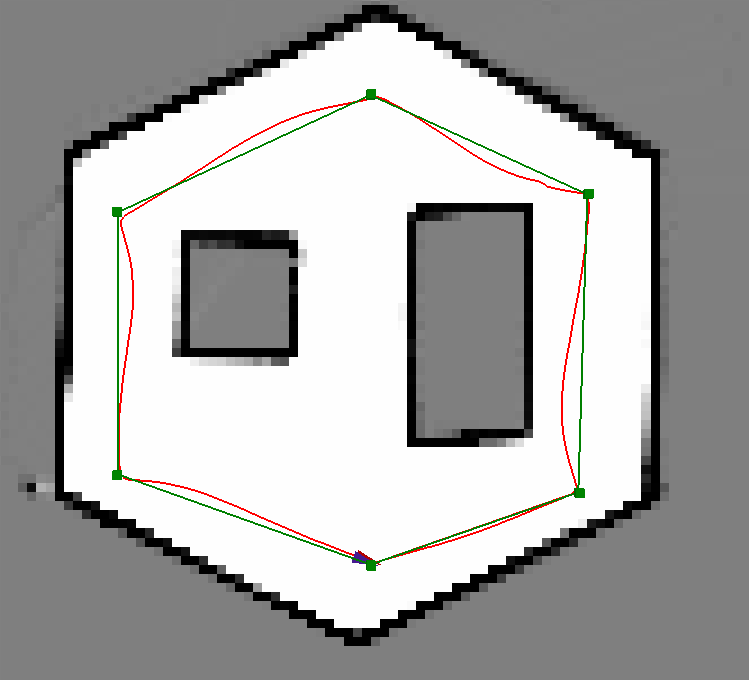
\includegraphics[width=0.65\linewidth]{obstacle_slam_10mx10m_5cm-map.png}
                \caption{Map built on the log file obstacle\_slam\_10mx10m\_5cm.log using the occupancy grid mapping algorithm. True pose of the robot is shown in red, and the desired path in green.}
                \label{fig:map}
            \end{figure}
    
        \subsubsection{Monte Carlo Localization Accuracy}
        
            Figure \ref{fig:localization} shows the robots pose over time on one of the provided log files. Here we see that the path of the robot as estimated by our localization routine is closed to the true pose as measured by motion capture. We quantified this by computing statistics of the pose error, which shows that our SLAM has an mean accuracy of \SI{4}{\centi\meter} whereas odometry has a mean accuracy of \SI{21}{\centi\meter}. We compute the distance between the true pose and point nearest in time from odometry and from SLAM, and Figure \ref{fig:localization_error} shows a plot of this error over time.
            
            \begin{figure}[h!]
                \centering
                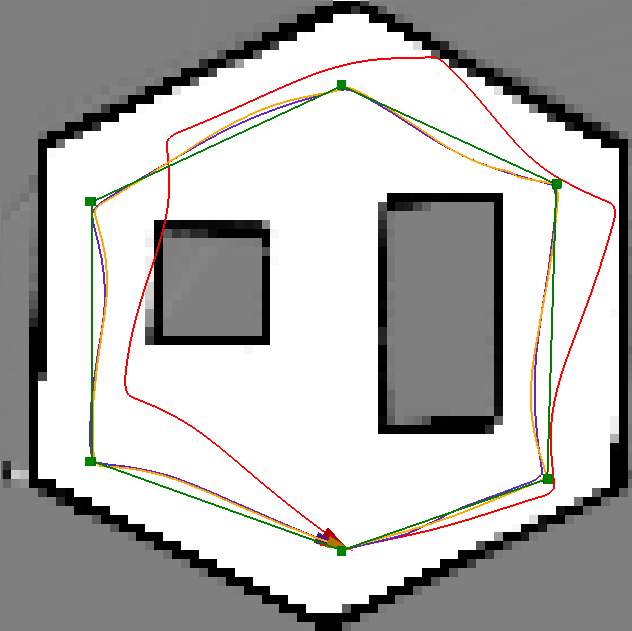
\includegraphics[width=0.65\linewidth]{obstacle_slam_10mx10m_5cm.png}
                \caption{Testing Localization only on obstacle\_slam\_10mx10m\_5cm.log, the green line is the plan, orange is the localized pose, and red is the odometry.}
                \label{fig:localization}
            \end{figure}
            
            \begin{figure}[h!]
                \centering
                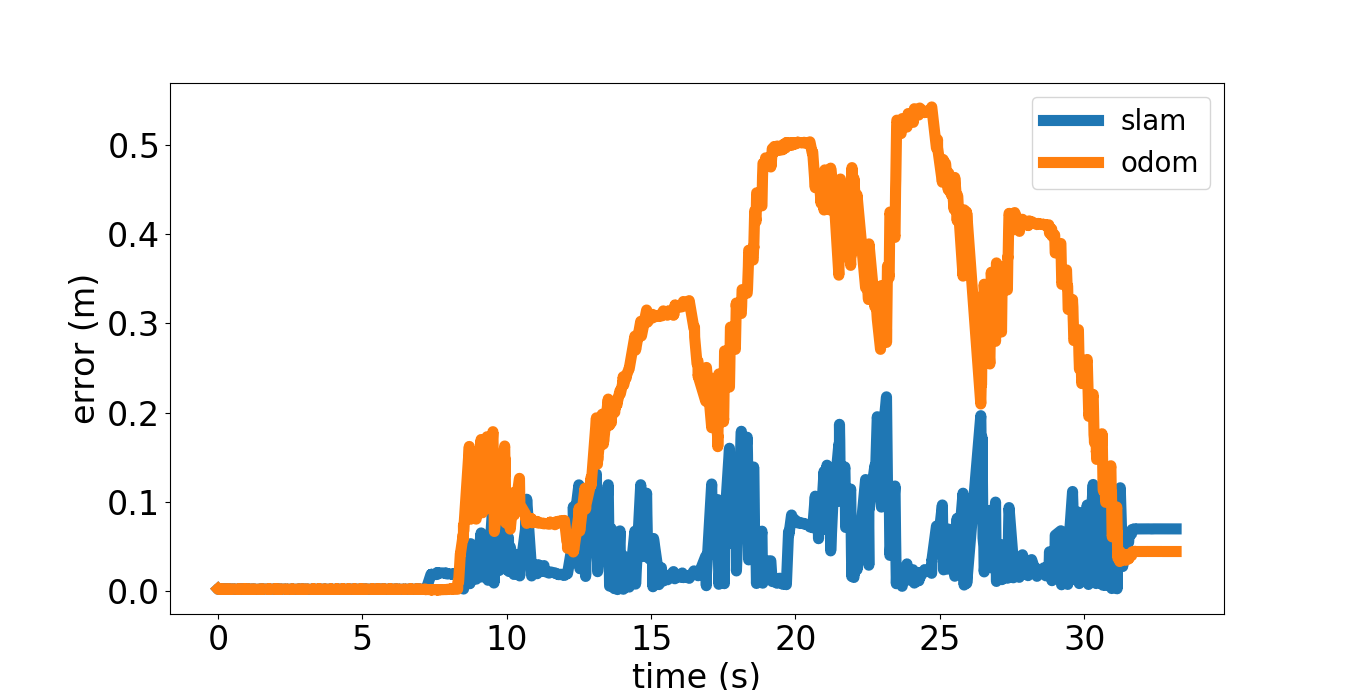
\includegraphics[width=1\linewidth]{localization_error.png}
                \caption{Error over time with respect to motion capture on the obstacle\_slam\_10mx10m\_5cm.log}
                \label{fig:localization_error}
            \end{figure}
            
            \begin{table}[h!]
                \centering
                \begin{tabular}{|c|c|c|c|} \hline
                  & Mean (cm) &   Std dev &   Max (cm) \\ \hline
                  Odometry & 20.8  & 18.6  &  54.2 \\ \hline
                  SLAM & 3.9 & 3.9 &  21.7 \\ \hline
                \end{tabular}
            \caption{Pose error statistics on obstacle\_slam\_10mx10m\_5cm.log}
                \label{tab:localization_error}
            \end{table}
            
            % ASSIGNED: Sid - explain the below plot!
            lorum ipsum verbatum lorum ipsum verbatum lorum ipsum verbatum lorum ipsum verbatum lorum ipsum verbatum lorum ipsum verbatum lorum ipsum verbatum lorum ipsum verbatum lorum ipsum verbatum lorum ipsum verbatum 
        
            \begin{figure}[H]
                \centering
                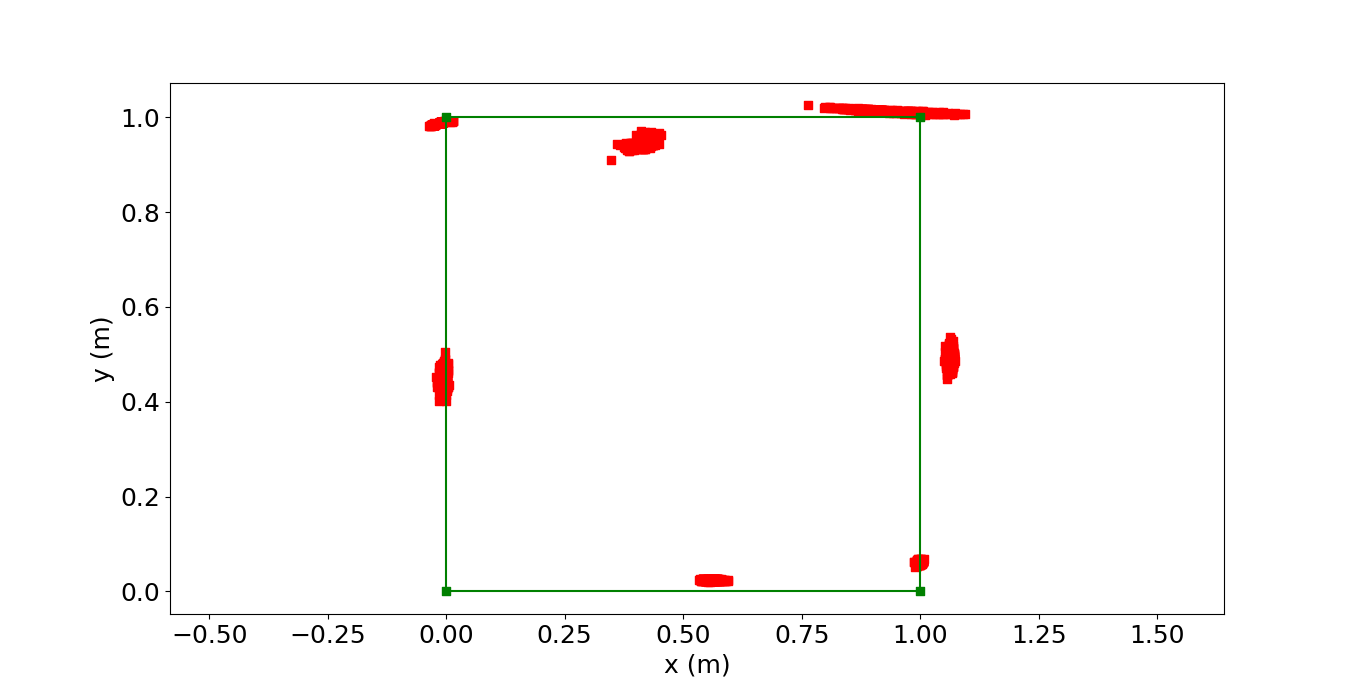
\includegraphics[width=1\linewidth]{drive_square_particles.png}
                \caption{Particles shown at various positions along a square path. Note that uncertainty is higher along the direction of motion.}
                \label{fig:square_particles}
            \end{figure}
    
        \subsubsection{Particle Filter Performance}
        
            It is essential that our SLAM system is fast enough to run in real time on our robot, otherwise the SLAM pose estimate will eventually lag behind our true pose. To quantify this, we measured how long it takes to update our particle filter for various numbers of particles. The timing results are shown in Table \ref{tab:filter_perf}. We fit a line to the data and calculated that we could handle $\approx400$ particles at \SI{10}{\hertz}.
    
            \begin{table}[h]
                \centering
                \begin{tabular}{|c|c|} \hline
                     \# Particles & Time (ms) \\    \hline
                     100 & 28 \\ \hline
                     200 & 48 \\ \hline
                     300 & 68 \\ \hline
                     500 & 126 \\ \hline
                     1000 & 250 \\ \hline
                \end{tabular}
                \caption{Time to update the particle filter. Each time was computed as the mean of 10 updates.}
                \label{tab:filter_perf}
            \end{table}
            
            \begin{figure}[h]
                \centering
                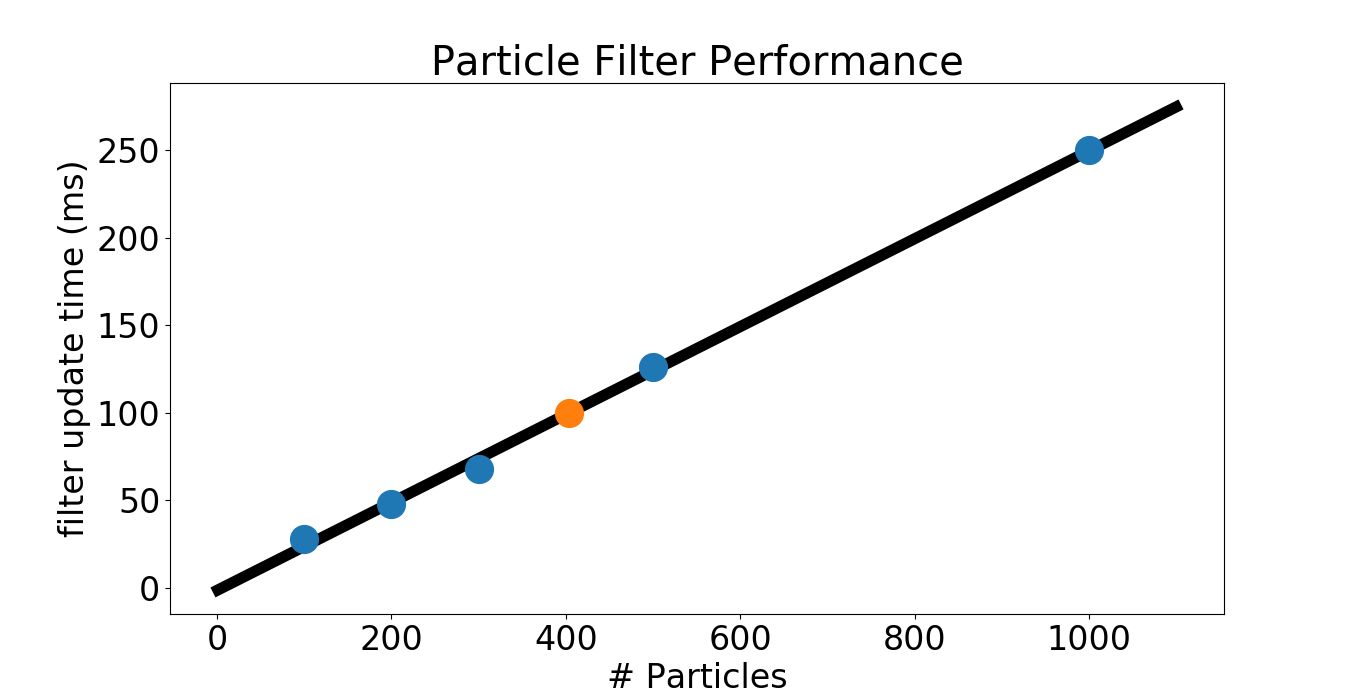
\includegraphics[width=0.85\linewidth]{filter_perf.png}
                \caption{Performance of the particle filter}
                \label{fig:perf}
            \end{figure}
            
        \subsubsection{Combined SLAM Accuracy}
        
            Finally, we measured the overall accuracy of our combined SLAM implementation. In this test, we drove the robot in four squares in the environment while running mapping and localization. Figure \ref{fig:slam_squares} shows the pose of the robot over time, and Figure \ref{fig:slam_squares_error} shows the error over time. Table \ref{tab:slam_error} shows the statistics of this error, which includes the mean error of \SI{6.5}{\centi\meter} for Odometry and \SI{7.4}{\centi\meter} for SLAM.
            
            \begin{figure}[ht]
                \centering
                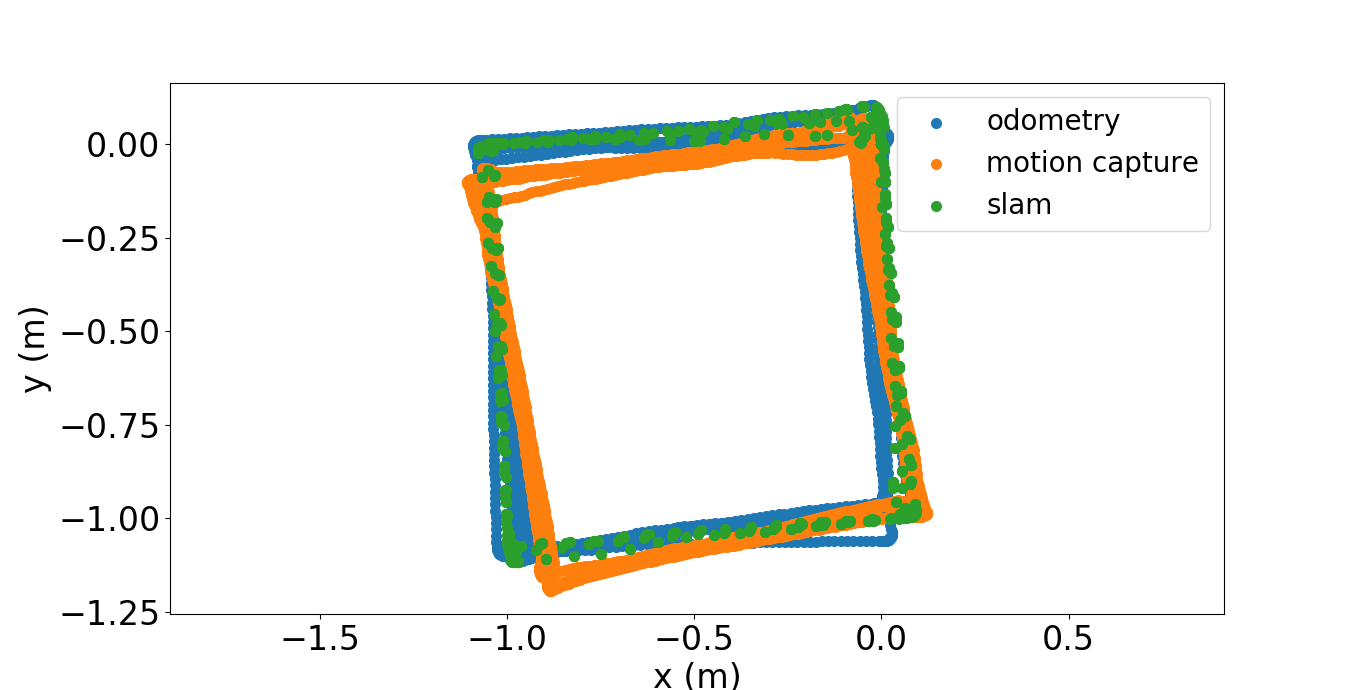
\includegraphics[width=1\linewidth]{slam_squares.png}
                \caption{SLAM Pose estimate versus motion capture pose}
                \label{fig:slam_squares}
            \end{figure}
            
            \begin{figure}[ht]
                \centering
                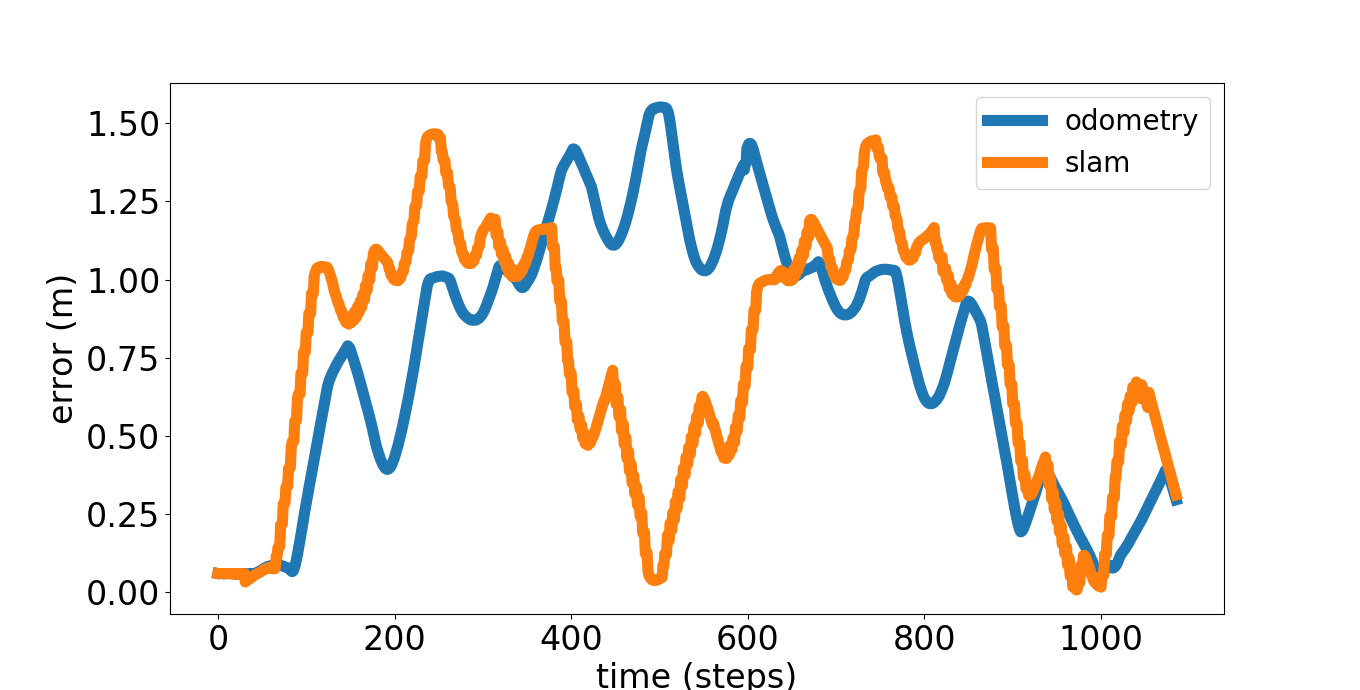
\includegraphics[width=1\linewidth]{slam_squares_error.png}
                \caption{Error over time with respect to motion capture}
                \label{fig:slam_squares_error}
            \end{figure}
            
            \begin{table}[ht]
                \centering
                \begin{tabular}{|c|c|c|c|c|} \hline
                  & Mean (cm) &   Std dev & N points & Max (cm) \\ \hline
                  Odometry & 6.5 & 2.5 & 1476 & 12.5 \\ \hline
                  SLAM & 7.4 & 3.9 & 1086 & 19.5 \\ \hline
                \end{tabular}
                \caption{Statistics of the pose error for four squares with full SLAM}
                \label{tab:slam_error}
            \end{table}
    
    \subsection{Planning and Exploration}
    
        \subsubsection{Path Planning}
        
            Our A star algorithm was able to correctly find the optimal path in all of the provided test environments. Furthermore, the mean planning time on the realistic maze scenario was \SI{2.625}{\milli\second}, which is faster then the update period of our SLAM algorithm ($\approx$\SI{100}{\milli\second}). Therefore, our planner is fast enough to operate every cycle if necessary.
            
            \begin{table}[h]
                \centering
                \begin{tabular}{|c|c|c|c|c|c|} \hline
                    & \multicolumn{5}{c|}{Planning Time (us)} \\ \hline
                    Environment & min & mean & max & median & stdev \\ \hline
                    convex & 194 & 197 & 218 & 195 & 7 \\ \hline
                    empty & 5332 & 5630 & 6171 & 5468 & 295 \\ \hline
                    maze & 2084 & 2625 & 3217 & 2533 & 410 \\ \hline
                    narrow & 5404 & 136776 & 271503 & 69468 & 131305 \\ \hline
                    wide & 5420 & 93529 & 268662 & 11361 & 122841 \\ \hline
                \end{tabular}
                \caption{A* Planning Times on the provided example problems. Statistics are computed on 20 trials on each map.}
                \label{tab:a_star_times}
            \end{table}
        
            After quantifying the performance of our A* planner, we tested the ability of our controller to follow the generates paths in with known map. In this experiment, we used the particle filter localization and manually selected a goal to plan our path. Figure \ref{fig:astar} shows the SLAM pose and motion capture pose of our robot as well as the path we intended to follow. Figure \ref{fig:astar_error} shows the error with respect to that path over time. 
            
            \begin{figure}[h]
                \centering
                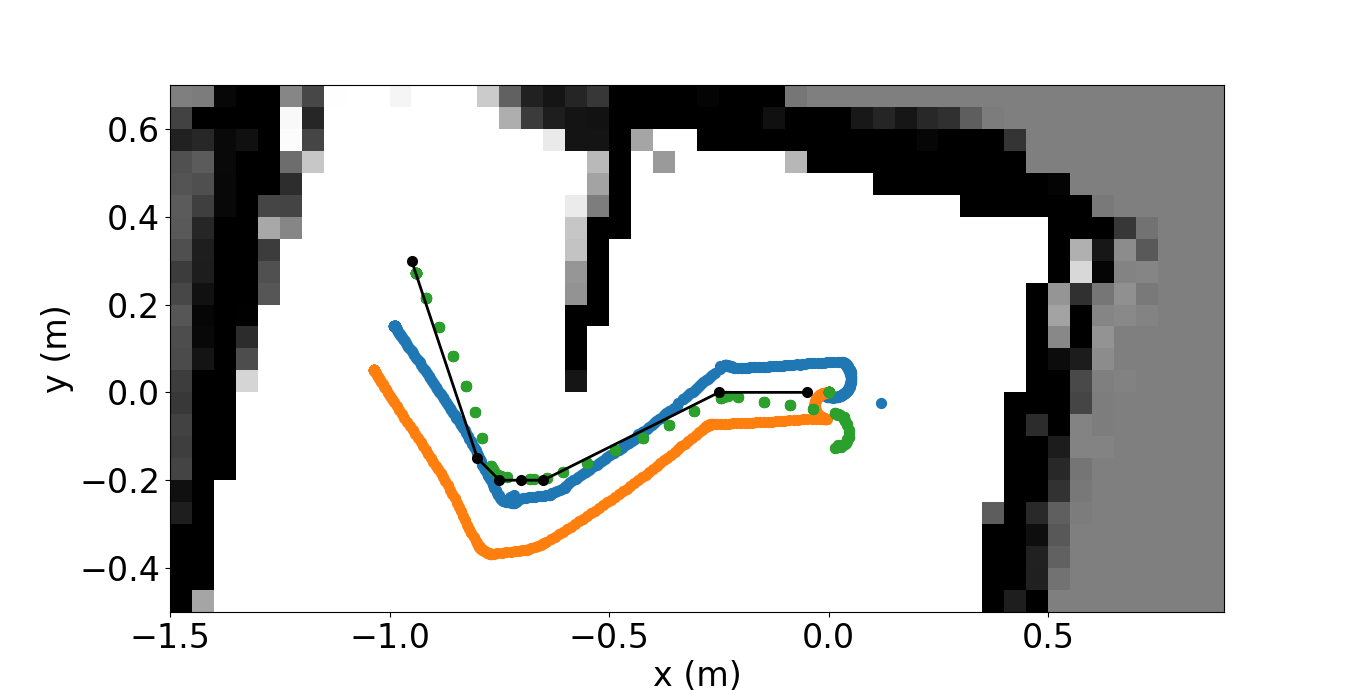
\includegraphics[width=1\linewidth]{astar.png}
                \caption{Position over time of slam pose (green) motion capture pose (blue) and odometry (orange) along with the planned path (black). In this example, the robot successfully avoids the obstacle.}
                \label{fig:astar}
            \end{figure}
            
            % \begin{figure}[h]
            %     \centering
            %     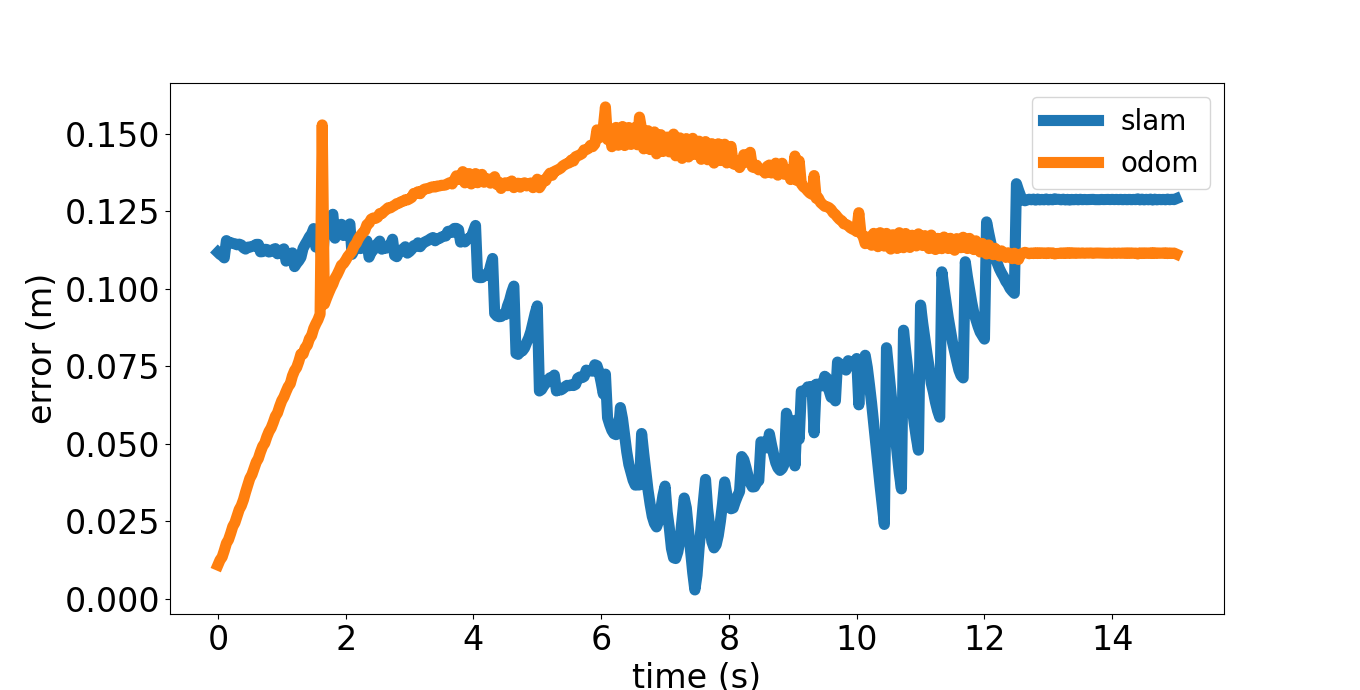
\includegraphics[width=1\linewidth]{astar_error.png}
            %     \caption{Position error over time of motion capture pose versus the planned path}
            %     \label{fig:astar_error}
            % \end{figure}
            
\section{Discussion}

    \subsection{Simultaneous Localization and Mapping (SLAM)}
    
        One interesting aspect of our results is that the localization accuracy does not appear to be higher than the accuracy of odometry in our full SLAM tests. However, we note that the accuracy of SLAM is quite similar to the accuracy of our localization only tests, where the error was roughly within \SI{5}{\centi\meter} and \SI{20}{\centi\meter}. This is consistent between those two test, however the odometry data is significantly more accurate in our full SLAM tests then in our localization only tests. In other words, our full SLAM system is as accurate in terms of position error as our localization system given a known map.

    \subsection{Planning and Exploration}
    
        In our experiments and in the final competition, we observed a several failures of our SLAM system in terms of choosing goals to navigate to and in actually navigating to those goals. We encountered several situations where the decision to select the furthest frontier first turned out to be a poor choice. For example, if there were two adjacent but distinct frontiers very far away and one frontier closer, the robot would begin to drive towards one of the further frontiers. Upon discovering that frontier, it would then plan a path back to the other frontier, only to then plan another path back to the second frontier. Ultimately, the intuition for choosing the furthest frontier first was wrong, and choosing the closest frontier would have potentially resulted in faster exploration.

        Another challenge was achieving smooth control between waypoints. When we first used our motion controller to follow paths, we noticed that the robot spent a lot of time turning to follow waypoints that are space very close together. This meant that the robot took a long time to follow a path. To mitigate this, we both increased the position and angle tolerance for intermediate waypoints and also chose to fix the forward speed when navigating to intermediate waypoints. This way the robot did not stop, in the event that the next waypoint is in a straight line, which was often the case in our experience, that path is execute more smoothly and more quickly.
    

\bibliographystyle{IEEEtran}
\bibliography{550-botlab}

\end{document}